\documentclass[a4paper]{article}
% \usepackage{a4wide,amssymb,epsfig,latexsym,multicol,array,hhline,fancyhdr}
\usepackage{amssymb,epsfig,latexsym,multicol,array,hhline,fancyhdr}
\usepackage{vntex}
\usepackage{amsmath}
\usepackage{lastpage}
\usepackage[lined,boxed,commentsnumbered]{algorithm2e}
\usepackage{enumerate}
\usepackage{color}
\usepackage{graphicx}
\usepackage{array}
\usepackage{tabularx, caption}
\usepackage{multirow}
\usepackage{multicol}
\usepackage{rotating}
\usepackage{graphics}
\usepackage{geometry}
\usepackage{pdflscape}
\usepackage{setspace}
\usepackage{xcolor}
\usepackage{epsfig}
\usepackage{tikz}
\usepackage{float}
\usepackage{longtable}
\usetikzlibrary{arrows,snakes,backgrounds}
\usepackage{makecell}
\usepackage{pifont}
\usepackage{enumitem}
\usepackage{booktabs}

% --- QUAN TRỌNG: Xóa hết các dòng hyperref cũ và chỉ giữ lại đúng 1 dòng này Ở CUỐI ---
\usepackage[linkcolor=blue, citecolor=green, urlcolor=blue]{hyperref}
% --------------------------------------------------------------------------------------

%\usepackage{pstcol}

\newtheorem{theorem}{{\bf Theorem}}
\newtheorem{property}{{\bf Property}}
\newtheorem{proposition}{{\bf Proposition}}
\newtheorem{corollary}[proposition]{{\bf Corollary}}
\newtheorem{lemma}[proposition]{{\bf Lemma}}

\newcommand\tab[1][14.5pt]{\hspace*{#1}}

\AtBeginDocument{\renewcommand*\contentsname{Mục Lục}}
\AtBeginDocument{\renewcommand*\listfigurename{Danh mục bảng và hình vẽ}}
\AtBeginDocument{\renewcommand*\refname{Tài liệu tham khảo}}

\setlength{\headheight}{40pt}
\pagestyle{fancy}
\fancyhead{} 
\fancyhead[L]{
 \begin{tabular}{rl}
    \begin{picture}(25,15)(0,0)
    \put(0,-8){
\includegraphics[width=8mm, height=8mm]{hcmut.png}}
   \end{picture}&
    \begin{tabular}{l}
        \textbf{\bf \ttfamily Trường Đại học Bách khoa -- ĐHQG-HCM}\\
        \textbf{\bf \ttfamily Khoa Khoa học ứng dụng}
    \end{tabular}   
 \end{tabular}
}
\fancyhead[R]{
    \begin{tabular}{l}
        \tiny \bf \\
        \tiny \bf 
    \end{tabular}  }
\fancyfoot{} 
\fancyfoot[L]{\scriptsize \ttfamily Bài tập lớn -- Vật lý đại cương A1 -- Học kỳ 252}
\fancyfoot[R]{\scriptsize \ttfamily Trang {\thepage}/\pageref{LastPage}}
\renewcommand{\headrulewidth}{0.3pt}
\renewcommand{\footrulewidth}{0.3pt}

%%%
\setcounter{secnumdepth}{4}
\setcounter{tocdepth}{3}
\makeatletter
\newcounter {subsubsubsection}[subsubsection]
\renewcommand\thesubsubsubsection{\thesubsubsection .\@alph\c@subsubsubsection}
\newcommand\subsubsubsection{\@startsection{subsubsubsection}{4}{\z@}%
                                     {-3.25ex\@plus -1ex \@minus -.2ex}%
                                     {1.5ex \@plus .2ex}%
                                     {\normalfont\normalsize\bfseries}}
\newcommand*\l@subsubsubsection{\@dottedtocline{3}{10.0em}{4.1em}}
\newcommand*{\subsubsubsectionmark}[1]{}
\makeatother

\usepackage{caption}
\captionsetup[figure]{labelsep=colon, font=small, labelfont=bf}

\hypersetup{
    colorlinks=true,
    linkcolor=black, % Đổi thành blue nếu muốn link có màu xanh nhưng không có khung
    citecolor=black,
    urlcolor=blue,
    pdfborder={0 0 0} % Triệt tiêu hoàn toàn khung bao quanh link
}

\usepackage[titles]{tocloft}

% --- Cấu hình in đậm cho Danh mục Hình vẽ ---
\renewcommand{\cftfigpresnum}{\bfseries Hình } % Đã bao gồm in đậm số thứ tự
\renewcommand{\cftfigaftersnum}{\bfseries :}    % In đậm dấu ":"
\renewcommand{\cftfigpagefont}{\bfseries}       % In đậm số trang

% Cân chỉnh khoảng cách để không bị đè chữ
\newlength{\figlabelwidth}
\settowidth{\figlabelwidth}{\bfseries Hình 99: } 
\addtolength{\cftfignumwidth}{\figlabelwidth}

% --- Cấu hình in đậm cho Danh mục Bảng biểu ---
\renewcommand{\cfttabpresnum}{\bfseries Bảng }
\renewcommand{\cfttabaftersnum}{\bfseries :}
\renewcommand{\cfttabpagefont}{\bfseries} 

\newlength{\tablabelwidth}
\settowidth{\tablabelwidth}{\bfseries Bảng 99: }
\addtolength{\cfttabnumwidth}{\tablabelwidth}


\usepackage{listings}
\usepackage{xcolor}

% Cấu hình màu sắc cho code
\definecolor{codegreen}{rgb}{0,0.6,0}
\definecolor{codegray}{rgb}{0.5,0.5,0.5}
\definecolor{codepurple}{rgb}{0.58,0,0.82}
\definecolor{backcolour}{rgb}{0.95,0.95,0.92}

% Thiết lập style cho Python
\lstdefinestyle{pythonstyle}{
    backgroundcolor=\color{backcolour},   
    commentstyle=\color{codegreen},
    keywordstyle=\color{magenta},
    numberstyle=\tiny\color{codegray},
    stringstyle=\color{codepurple},
    basicstyle=\ttfamily\footnotesize,
    breakatwhitespace=false,         
    breaklines=true,                 
    captionpos=b,                    
    keepspaces=true,                 
    numbers=left,                    
    numbersep=5pt,                  
    showspaces=false,                
    showstringspaces=false,
    showtabs=false,                  
    tabsize=2,
    language=Python
}




\begin{document}

\begin{titlepage}
\begin{center}
\textbf{ĐẠI HỌC QUỐC GIA THÀNH PHỐ HỒ CHÍ MINH \\
TRƯỜNG ĐẠI HỌC BÁCH KHOA} \\
\textbf{KHOA KHOA HỌC ỨNG DỤNG}
\end{center}

\vspace{1cm}

\begin{figure}[h!]
\begin{center}

\includegraphics[width=3cm]{hcmut.png}
\end{center}
\end{figure}

\vspace{1cm}


\begin{center}
\begin{tabular}{c}
\multicolumn{1}{c}{\textbf{{\LARGE VẬT LÝ ĐẠI CƯƠNG A1 (PH1003)}}}\\
~~\\
\hline
\\
\multicolumn{1}{l}{\textbf{{\Large BÀI TẬP LỚN}}}\\
\\
\textbf{{\large \MakeUppercase{Mô phỏng sự phân bố năng lượng điện trường} }}
\\
\textbf{{\large \MakeUppercase{và mật độ năng lượng trong tụ điện phẳng}}}\\
\\
\\
\hline
\end{tabular}
\end{center}

\vspace{1cm}

\begin{table}[h]
\begin{tabular}{rrl}
\hspace{3 cm} & \textbf{Giảng viên hướng dẫn:} &TS.Trịnh Trần Hồng Duyên\\

& \textbf{Sinh viên thực hiện:} & \textbf{Trần Đăng Bảo - 2210270} \\
& & Trần Minh Khôi - 2311703 \\
& & Mai Trần Thiên Ân - 2310181 \\ 
& & Nguyễn Quốc Trạng  - 2213565 \\
& & Võ Thanh Quân - 2114562\\
& & Thịnh Trần Khánh Linh - 2211862\\
& & Trần Nguyễn Phương Tuyền - 2213833\\
\end{tabular}
\end{table}

\vspace{1cm}
\begin{center}
{TP. Hồ Chí Minh -- 2026}
\end{center}
\end{titlepage}
\thispagestyle{empty}

%\thispagestyle{empty}

\newpage
\tableofcontents
\thispagestyle{empty}
\newpage
\listoffigures
\addcontentsline{toc}{section}{\listfigurename} 
\thispagestyle{empty}
\newpage
\setcounter{page}{1}

%%%%%%%%%%%%%%%%%%%%%%%%%%%%%%%%%
\section*{Danh sách thành viên và phân chia công việc}

\begin{center}
\begin{tabular}{|c|c|c|c|c|}
\hline
\textbf{STT} & \textbf{Họ tên} & \textbf{MSSV} & \makecell[c]{\textbf{Công việc}} & \makecell[c]{\textbf{Phần trăm} \\ \textbf{hoàn thành}}\\
\hline 
%%%%Student 1%%%%%%%%%%
\multirow{3}{*}{1} & \multirow{3}{*}{Trần Đăng Bảo} & \multirow{3}{*}{2210270} &  & \multirow{3}{*}{100\%}\\
 & &  &  &\\
 & &  &  &\\
\hline 
%%%%Student 2%%%%%%%%%%%
\multirow{3}{*}{2} & \multirow{3}{*}{Trần Minh Khôi} & \multirow{3}{*}{2311703} &  & \multirow{3}{*}{100\%}\\
 & &  &  &\\
 & &  &  &\\
\hline
%%%%Student 3%%%%%%%%%%%
\multirow{3}{*}{3} & \multirow{3}{*}{Mai Trần Thiên Ân} & \multirow{3}{*}{2310181} &  & \multirow{3}{*}{100\%}\\
 & &  &  &\\
 & &  &  &\\
\hline
%%%%Student 4%%%%%%%%%%%
\multirow{3}{*}{4} & \multirow{3}{*}{Nguyễn Quốc Trạng } & \multirow{3}{*}{2213565} &  & \multirow{3}{*}{100\%}\\
 & &  &  &\\
 & &  &  &\\
\hline
%%%%Student 5%%%%%%%%%%%
\multirow{3}{*}{5} & \multirow{3}{*}{Võ Thanh Quân} & \multirow{3}{*}{2114562} &  & \multirow{3}{*}{100\%}\\
 & &  &  &\\
 & &  &  &\\
\hline
%%%%Student 6%%%%%%%%%%%
\multirow{3}{*}{5} & \multirow{3}{*}{Thịnh Trần Khánh Linh} & \multirow{3}{*}{2211862} &  & \multirow{3}{*}{100\%}\\
 & &  &  &\\
 & &  &  &\\
\hline
%%%%Student 7%%%%%%%%%%%
\multirow{3}{*}{5} & \multirow{3}{*}{Trần Nguyễn Phương Tuyền} & \multirow{3}{*}{2213833} &  & \multirow{3}{*}{100\%}\\
 & &  &  &\\
 & &  &  &\\
\hline


\end{tabular}
\end{center}

%%%%%%%%%%%%%%%%%%%%%%%%%%%%%%%%%
\newpage

\section{Cơ sở lý thuyết}
\subsection{Tụ điện}
\subsubsection{Cấu tạo}
Một tụ điện (capacitor) gồm có 2 vật dẫn như hình vẽ. Các vật dẫn này được gọi là các
bản tụ (plate). Khi vật dẫn được tích điện, các bản tụ sẽ mang điện tích bằng nhau về độ
lớn nhưng ngược dấu. Hiệu điện thế tồn tại giữa các bản tụ gây ra bởi các điện tích.

\begin{figure}[H]
    \centering
    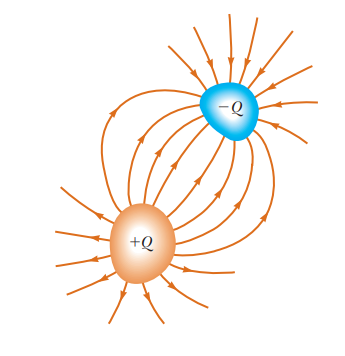
\includegraphics[width=0.4\linewidth]{images/figure1.png}
    \caption{Biểu diễn sơ đồ điện trường của một tụ điện bất kỳ, gồm hai vật dẫn mang điện lượng bằng nhau nhưng trái dấu ($+Q$ và $-Q$)}
    \label{fig:placeholder}
\end{figure}

\subsubsection{Định nghĩa}
Khi vật dẫn $B$ bao trùm hết vật dẫn $A$, ta tích cho vật dẫn $A$ một điện tích $+Q$, thì hai bề mặt trong và ngoài của vật dẫn $B$ sẽ tích điện $-Q$, $+Q$. Nối mặt ngoài cùng của vật dẫn $B$ xuống đất (mặt ngoài cùng trung hòa) ta có hai bề mặt kim loại tích điện trái dấu $-Q$, $+Q$ gọi là hai bản (cốt) của tụ điện.

\begin{figure}[H]
    \centering
    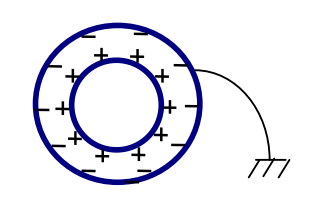
\includegraphics[width=0.5\linewidth]{images/figure2.png}
    \caption{Mô hình cấu tạo tụ điện: Vật dẫn bao ngoài được nối đất để triệt tiêu điện tích cùng dấu, tạo thành hai bản tụ mang điện tích trái dấu có độ lớn bằng nhau.}
    \label{fig:placeholder}
\end{figure}

\subsubsection{Điện dung của tụ điện}
Khi ta tích điện cho một tụ điện điện lượng $Q$, giữa hai bản tụ sẽ xuất hiện một hiệu điện thế $\Delta V$. Nếu tiếp tục tăng điện tích $Q$ thì hiệu điện thế $\Delta V$ cũng tăng theo tỉ lệ thuận tương ứng. Tuy nhiên, tỉ số giữa độ lớn điện tích $Q$ và hiệu điện thế $\Delta V$ luôn luôn là một hằng số đối với một tụ điện nhất định.

Hằng số này đặc trưng cho khả năng tích điện của tụ điện ở một hiệu điện thế cho trước, và được gọi là điện dung của tụ điện.

Biểu thức định nghĩa điện dung: 
$$C = \frac{Q}{\Delta V}$$

Trong đó: 
\begin{itemize}
\item $C$: Điện dung của tụ điện, có đơn vị là Farad (F).
\item $Q$: Độ lớn điện tích trên một bản tụ, có đơn vị là Coulomb (C).
\item $\Delta V$: Hiệu điện thế giữa hai bản tụ, có đơn vị là Volt (V).
\end{itemize}

\subsubsection{Tụ điện phẳng}
\begin{figure}[H]
    \centering
    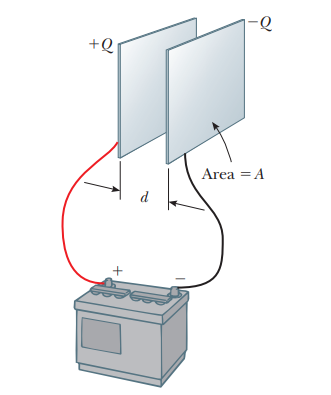
\includegraphics[width=0.4\linewidth]{images/figure3.png}
    \caption{Cấu tạo cơ bản của tụ điện phẳng: Hai bản kim loại có cùng diện tích bề mặt $A$, đặt cách nhau một khoảng $d$ và mang điện lượng trái dấu ($+Q$ và $-Q$) khi được nạp điện.}
    \label{fig:placeholder}
\end{figure}
Tụ điện phẳng là một trong những cấu trúc cơ bản và mang tính nền tảng nhất trong nghiên cứu tĩnh điện học. Cấu tạo không gian của hệ thống này bao gồm hai bản kim loại phẳng có cùng diện tích bề mặt $A$, được bố trí song song với nhau và ngăn cách bởi một khoảng cách $d$ trong môi trường chân không (hoặc không khí). Quá trình nạp điện cho hệ thống dẫn đến sự phân bố điện tích đối xứng, trong đó một bản mang điện tích dương $+Q$ và bản đối diện mang điện tích âm $-Q$. Hệ quả của quá trình này là sự hình thành mật độ điện tích mặt $\sigma$ trên bề mặt mỗi bản kim loại, được xác định bởi tỷ số giữa lượng điện tích và diện tích bề mặt tương ứng:
$$\sigma = \frac{Q}{A}$$

Trong các khảo sát lý thuyết, một giả thiết lý tưởng hóa thường được áp dụng là khoảng cách $d$ rất nhỏ so với kích thước tuyến tính của các bản tụ. Giả thiết này đóng vai trò quan trọng trong việc loại bỏ ảnh hưởng của hiệu ứng mép tại các rìa vật dẫn, cho phép xem xét điện trường $\vec{E}$ nội bộ giữa hai bản tụ là một điện trường đều, đồng thời coi điện trường ở không gian bên ngoài hệ thống xấp xỉ bằng $0$. Dựa trên cơ sở đó và thông qua việc áp dụng định lý Gauss, độ lớn của cường độ điện trường đều bên trong khoảng không gian giữa hai bản tụ được xác định chặt chẽ bằng biểu thức:
$$E = \frac{\sigma}{\epsilon_0} = \frac{Q}{\epsilon_0 A}$$
\textit{(Với $\epsilon_0$ là hằng số điện của chân không).}

Do đặc tính phân bố đều của điện trường nội bộ, độ giảm thế (hay hiệu điện thế $\Delta V$) giữa hai bản vật dẫn thể hiện mối quan hệ tuyến tính với chiều dài đường sức $d$. Mối liên hệ này được biểu diễn qua phương trình:
$$\Delta V = E \cdot d = \frac{Q \cdot d}{\epsilon_0 A}$$

Bằng cách tích hợp biểu thức hiệu điện thế này vào định nghĩa tổng quát của điện dung, biến số $Q$ được triệt tiêu, từ đó thiết lập được hệ thức toán học tính toán điện dung dành riêng cho cấu trúc tụ điện phẳng:
$$C = \frac{Q}{\Delta V} = \frac{\epsilon_0 A}{d}$$

Việc thiết lập phương trình giải tích trên đã minh chứng cho một nguyên lý vật lý cốt lõi: điện dung của một tụ điện phẳng mang tính chất nội tại và hoàn toàn độc lập với lượng điện tích $Q$ mà hệ đang lưu trữ hay hiệu điện thế $\Delta V$ được áp đặt lên nó. Thực chất, đại lượng này được quyết định hoàn toàn bởi các thông số cấu trúc không gian của hệ thống - tỷ lệ thuận với diện tích bề mặt bản tụ $A$, tỷ lệ nghịch với khoảng cách $d$ - và bản chất của môi trường điện môi tồn tại giữa hai bản cực.

\subsubsection{Sự phụ thuộc của điện dung vào các yếu tố hình học}
Từ biểu thức tính điện dung của tụ điện phẳng ($C = \frac{\epsilon_0 A}{d}$), ta có thể giải thích bản chất vật lý của sự phụ thuộc này thông qua các đặc điểm sau:
\begin{enumerate}
    \item Ảnh hưởng của diện tích bản tụ ($A$)\\
    Khi tụ điện được nạp điện từ một nguồn, các electron sẽ di chuyển và tích tụ trên bản cực âm, đồng thời bản cực dương mất đi một lượng electron tương ứng. Nếu diện tích bề mặt bản tụ $A$ càng lớn, không gian để điện tích phân bố càng rộng rãi. Điều này cho phép các bản tụ chứa được một lượng điện tích lớn hơn nhiều mà vẫn duy trì cùng một mức hiệu điện thế. Do đó, điện dung của tụ điện tỉ lệ thuận với diện tích bề mặt bản tụ ($C \propto A$).
    \item Ảnh hưởng của khoảng cách giữa hai bản tụ ($d$)\\
    Xét trường hợp tụ điện đang được duy trì kết nối với một nguồn điện (pin). Giả sử ta dịch chuyển để đưa hai bản tụ lại gần nhau (làm giảm khoảng cách $d$).
    \begin{itemize}
        \item Ngay tại khoảnh khắc dịch chuyển, lượng điện tích trên các bản tụ chưa kịp thay đổi tức thời, do đó cường độ điện trường $E$ giữa hai bản tạm thời giữ nguyên.
        \item Tuy nhiên, vì khoảng cách $d$ giảm, hiệu điện thế giữa hai bản tụ lúc này (tính theo công thức $\Delta V = E \cdot d$) sẽ bị suy giảm, trở nên nhỏ hơn hiệu điện thế của nguồn pin.
    \end{itemize}
\end{enumerate}

Sự chênh lệch điện áp này ngay lập tức tạo ra một điện trường dọc theo các dây nối, thúc đẩy dòng điện tích tiếp tục di chuyển từ nguồn vào tụ điện. Quá trình này làm tăng lượng điện tích $Q$ trên các bản tụ, kéo theo sự gia tăng hiệu điện thế giữa chúng. Dòng điện tích sẽ chỉ dừng lại khi hiệu điện thế của tụ điện phục hồi và cân bằng hoàn toàn với hiệu điện thế của pin.

Như vậy, thao tác đưa hai bản cực lại gần nhau đã giúp tụ điện gia tăng khả năng tích trữ điện tích ở cùng một mức điện áp. Ngược lại, nếu khoảng cách $d$ tăng lên, lượng điện tích lưu trữ sẽ giảm đi. Điều này giải thích bản chất vật lý của mối quan hệ tỉ lệ nghịch giữa điện dung $C$ và khoảng cách $d$ ($C \propto \frac{1}{d}$).

\subsection{Cường độ điện trường trong tụ điện phẳng}
\subsubsection{Định lý Gauss}
Định lý Gauss trong tĩnh điện học phát biểu rằng: Thông lượng điện trường gửi qua một mặt kín bất kỳ (gọi là mặt Gauss) bằng tổng đại số các điện tích nằm trọn bên trong mặt đó chia cho hằng số điện của chân không.

Biểu thức toán học:
$$\Phi_E = \oint \vec{E} \cdot d\vec{A} = \frac{q_{in}}{\epsilon_0}$$

Trong đó:
\begin{itemize}
    \item $\Phi_E$: Thông lượng điện trường qua mặt kín.
    \item $\vec{E}$: Vectơ cường độ điện trường tại vị trí vi phân diện tích.
    \item $q_{in}$: Tổng đại số các điện tích được bao bọc bên trong mặt Gauss.
    \item $\epsilon_0$: Hằng số điện của chân không.
\end{itemize}

Nguyên tắc chọn mặt Gauss:

Mặc dù định lý Gauss đúng với mọi mặt kín, nhưng trong thực hành, để tính toán cường độ điện trường $\vec{E}$ một cách dễ dàng, ta cần chọn một mặt Gauss phù hợp dựa trên tính đối xứng của sự phân bố điện tích. Bề mặt được chọn cần thỏa mãn ít nhất một trong các điều kiện sau đây để đơn giản hóa quá trình lấy tích phân:
\begin{enumerate}
    \item \textbf{Tính đối xứng về độ lớn:} Độ lớn cường độ điện trường $E$ không đổi tại mọi điểm trên bề mặt.
    \item \textbf{Điện trường vuông góc với mặt phẳng:} Vectơ điện trường $\vec{E}$ song song với vectơ diện tích $d\vec{A}$. Khi đó, biểu thức dưới dấu tích phân trở thành vô hướng: $\vec{E} \cdot d\vec{A} = E dA$.
    \item \textbf{Điện trường tiếp tuyến với mặt phẳng:} Vectơ điện trường $\vec{E}$ vuông góc với vectơ diện tích $d\vec{A}$. Khi đó, tích vô hướng triệt tiêu: $\vec{E} \cdot d\vec{A} = 0$.
    \item \textbf{Vùng không có điện trường:} Cường độ điện trường bằng không tại mọi điểm trên bề mặt xét ($E = 0$).
\end{enumerate}


\subsubsection{Xác định cường độ điện trường bằng định lý Gauss}
Để xác định cường độ điện trường trong tụ điện phẳng, quy trình tính toán được thực hiện qua hai giai đoạn: xác định điện trường do một bản phẳng đơn lẻ gây ra và áp dụng nguyên lý chồng chất cho hệ hai bản tụ.

\textbf{Cường độ điện trường của một bản phẳng tích điện}
    
Xét một bản kim loại phẳng vô hạn, tích điện đều với mật độ điện tích mặt $\sigma$. Chọn mặt Gauss là một hình trụ có trục vuông góc với bản tích điện và hai đáy song song với bản đó. Do tính đối xứng, vectơ cường độ điện trường $\vec{E}$ có hướng vuông góc với bản kim loại và độ lớn bằng nhau tại mọi điểm trên hai mặt đáy của hình trụ. Trong khi đó, thông lượng điện trường qua mặt xung quanh của hình trụ bằng không vì các đường sức song song với bề mặt này.

Áp dụng định lý Gauss, thông lượng điện trường chỉ đi qua hai mặt đáy, dẫn đến biểu thức xác định cường độ điện trường do một bản phẳng gây ra có độ lớn:
$$E = \frac{\sigma}{2\epsilon_0}$$

\textbf{Cường độ điện trường bên trong và bên ngoài tụ điện}

Xét mô hình tụ điện phẳng gồm hai bản kim loại song song mang điện tích trái dấu với mật độ $\sigma$ và $-\sigma$. Theo nguyên lý chồng chất, cường độ điện trường tại một điểm bất kỳ là tổng vectơ của điện trường do từng bản cực tạo ra.

\begin{itemize}
    \item \textbf{Vùng không gian giữa hai bản tụ:} Các vectơ điện trường do bản dương và bản âm gây ra có cùng phương và cùng hướng. Do đó, chúng cộng đại số với nhau, tạo ra điện trường bên trong tụ điện có độ lớn không đổi:
    $$E = \frac{\sigma}{2\epsilon_0} + \frac{\sigma}{2\epsilon_0} = \frac{\sigma}{\epsilon_0}$$
    \item \textbf{Vùng không gian bên ngoài tụ điện:} Vectơ điện trường do hai bản cực gây ra có cùng độ lớn nhưng ngược chiều nhau. Hệ quả là chúng triệt tiêu lẫn nhau, khiến cường độ điện trường ở vùng này xấp xỉ bằng không.
\end{itemize}

\textbf{Điều kiện áp dụng mô hình lý tưởng}

Các kết quả phân tích trên được thiết lập dựa trên mô hình tụ điện lý tưởng, trong đó thỏa mãn các điều kiện sau: diện tích của hai bản tụ đủ lớn để có thể coi là vô hạn, khoảng cách $d$ giữa hai bản rất nhỏ so với kích thước tuyến tính của chúng, và có thể bỏ qua hiệu ứng mép tại các rìa bản tụ.

\subsection{Năng lượng và mật độ năng lượng điện trường}
Việc tách biệt các điện tích dương và âm trong hệ thống hai vật dẫn của tụ điện đòi hỏi một công cơ học nhất định. Công này không mất đi mà được lưu trữ trong hệ thống dưới dạng năng lượng tiềm tàng, cụ thể là năng lượng tĩnh điện. Khi tụ điện được phóng điện thông qua một dây dẫn, năng lượng này sẽ được giải phóng, đôi khi có thể quan sát được dưới dạng tia lửa điện hoặc gây ra hiện tượng giật điện nếu tiếp xúc trực tiếp.

\begin{figure}
    \centering
    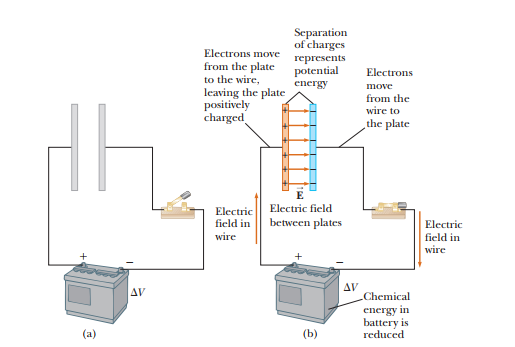
\includegraphics[width=0.7\linewidth]{images/figure4.png}
    \caption{Sơ đồ mô tả quá trình nạp điện và chuyển hóa năng lượng trong tụ điện phẳng: (a) Khi mạch hở; (b) Khi đóng công tắc, năng lượng hóa học từ pin chuyển hóa thành năng lượng điện thế thông qua sự phân tách các điện tích và thiết lập điện trường $\vec{E}$ giữa hai bản tụ.}
    \label{fig:placeholder}
\end{figure}
\subsubsection{Tính toán năng lượng lưu trữ trong tụ điện}
Để xác định tổng năng lượng tích lũy, ta xem xét quá trình nạp điện cho tụ điện như một chuỗi các bước dịch chuyển điện tích vi phân. Giả sử tại một thời điểm bất kỳ trong quá trình nạp, điện tích trên tụ điện là $q$ và hiệu điện thế tương ứng là $\Delta V$. Theo định nghĩa về điện dung, ta có mối liên hệ:
$$\Delta V = \frac{q}{C}$$

Khi một lượng điện tích vi phân $dq$ được chuyển từ bản mang điện thế thấp sang bản mang điện thế cao hơn, công vi phân $dW$ cần thực hiện để thắng lực điện trường là:
$$dW = \Delta V dq = \frac{q}{C}dq$$

Tổng công cần thiết để nạp điện cho tụ điện từ trạng thái không tích điện ($q=0$) đến khi đạt điện tích cuối cùng $Q$ được xác định bằng phép tính tích phân:
$$W = \int_{0}^{Q} \frac{q}{C} dq = \frac{1}{C} \int_{0}^{Q} q \, dq = \frac{Q^2}{2C}$$

\begin{figure}[H]
    \centering
    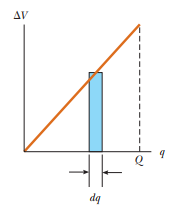
\includegraphics[width=0.35\linewidth]{images/figure5.png}
    \caption{Mối liên hệ tuyến tính giữa hiệu điện thế và điện tích của tụ điện. Tổng công thực hiện để nạp điện cho tụ đạt giá trị $Q$ tương ứng với diện tích hình tam giác nằm dưới đường thẳng $\Delta V(q)$.}
    \label{fig:placeholder}
\end{figure}

Vì công thực hiện bằng với năng lượng thế tĩnh điện $U$ tích lũy trong tụ điện, ta có các biểu thức tương đương để xác định năng lượng này:
$$U = \frac{Q^2}{2C} = \frac{1}{2}Q\Delta V = \frac{1}{2}C(\Delta V)^2$$

\subsubsection{Mật độ năng lượng điện trường}
Năng lượng trong tụ điện có thể được xem là lưu trữ trực tiếp trong điện trường tồn tại giữa hai bản cực. Đối với trường hợp tụ điện phẳng, ta có mối liên hệ giữa hiệu điện thế và cường độ điện trường là $\Delta V = Ed$, và điện dung $C = \frac{\epsilon_0 A}{d}$. Thay các giá trị này vào công thức năng lượng, ta thu được:
$$U = \frac{1}{2} \left( \frac{\epsilon_0 A}{d} \right) (Ed)^2 = \frac{1}{2} (\epsilon_0 Ad) E^2$$
Vì tích số $Ad$ chính là thể tích $V_{vol}$ của vùng không gian chứa điện trường, năng lượng trên mỗi đơn vị thể tích - gọi là mật độ năng lượng điện trường $u_E$ - được xác định như sau:
$$u_E = \frac{U}{Ad} = \frac{1}{2} \epsilon_0 E^2$$

Mặc dù biểu thức này được xây dựng dựa trên mô hình tụ điện phẳng, nó mang tính chất tổng quát và đúng cho bất kỳ điện trường nào trong chân không. Như vậy, mật độ năng lượng tại một điểm bất kỳ trong điện trường luôn tỷ lệ thuận với bình phương độ lớn cường độ điện trường tại điểm đó.

\subsection{Tụ điện phẳng có điện môi}
Chất điện môi là các vật liệu không dẫn điện, điển hình như cao su, thủy tinh hoặc giấy sáp. Việc đưa chất điện môi vào giữa các bản tụ không chỉ giúp ngăn cách vật lý giữa hai bản cực mà còn làm thay đổi đáng kể các đặc tính điện của hệ thống.
\subsubsection{Ảnh hưởng của điện môi lên điện dung}
\begin{figure}[H]
    \centering
    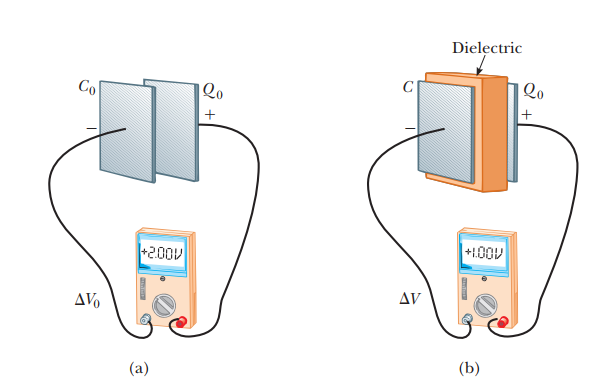
\includegraphics[width=0.6\linewidth]{images/figure6.png}
    \caption{Thí nghiệm minh họa ảnh hưởng của chất điện môi lên hiệu điện thế của tụ điện khi giữ nguyên điện lượng $Q_0$. (a) Hiệu điện thế ban đầu $\Delta V_0$ khi không có điện môi; (b) Hiệu điện thế $\Delta V$ giảm xuống sau khi chèn chất điện môi lấp đầy khoảng không gian giữa hai bản cực.}
    \label{fig:placeholder}
\end{figure}
Để khảo sát tác dụng của chất điện môi, xét một tụ điện phẳng đã được nạp điện lượng $Q_0$ và sau đó ngắt khỏi nguồn. Tại trạng thái ban đầu trong chân không, tụ điện có điện dung $C_0$ và hiệu điện thế đo được giữa hai bản tụ là $\Delta V_0 = Q_0/C_0$.

Khi chèn một tấm điện môi lấp đầy khoảng không gian giữa hai bản cực, thực nghiệm cho thấy hiệu điện thế giữa chúng giảm xuống một giá trị $\Delta V$ mới. Mối liên hệ giữa hiệu điện thế trước và sau khi có điện môi được xác định qua hệ số không thứ nguyên $\kappa$:
$$\Delta V = \frac{\Delta V_0}{\kappa}$$

Vì hệ thống đã được ngắt khỏi nguồn nên điện tích $Q_0$ trên các bản cực không thay đổi. Do đó, giá trị điện dung của tụ điện khi có điện môi phải thay đổi tương ứng:
$$C = \frac{Q_0}{\Delta V} = \frac{Q_0}{\Delta V_0 / \kappa} = \kappa \frac{Q_0}{\Delta V_0}$$
Hay:
$$C = \kappa C_0$$

Trong đó, $\kappa$ được gọi là hằng số điện môi của vật liệu. Vì thực nghiệm cho thấy $\Delta V < \Delta V_0$, ta luôn có $\kappa > 1$, nghĩa là việc chèn chất điện môi luôn làm tăng điện dung của tụ điện. Đối với mô hình tụ điện phẳng, biểu thức tính điện dung tổng quát khi có điện môi được xác định bởi:
$$C = \kappa \frac{\epsilon_0 A}{d}$$

\subsubsection{Giới hạn vật lý và điện áp định mức}
Mặc dù việc giảm khoảng cách $d$ hoặc tăng hằng số điện môi $\kappa$ có thể làm tăng điện dung, nhưng trong thực tế, các tham số này bị giới hạn bởi hiện tượng đánh thủng điện môi. Với mỗi loại vật liệu, tồn tại một giá trị cường độ điện trường tối đa mà nó có thể chịu đựng được trước khi mất tính cách điện và trở nên dẫn điện, gọi là độ bền điện môi.

Hệ quả là các tụ điện thực tế luôn đi kèm với thông số điện áp định mức (hoặc điện áp đánh thủng). Thông số này đại diện cho mức hiệu điện thế lớn nhất có thể đặt vào tụ điện mà không gây ra sự phóng điện xuyên qua lớp điện môi. Do đó, khi thiết kế và lựa chọn tụ điện cho các ứng dụng cụ thể, người kỹ sư cần phải xem xét đồng thời cả giá trị điện dung và giới hạn điện áp hoạt động để đảm bảo an toàn và độ bền cho hệ thống.

\newpage
\section{Mô phỏng}
\subsection{Mục đích và phạm vi mô phỏng}
\subsubsection{Mục đích mô phỏng}
Tiến trình mô phỏng được thiết lập với mục tiêu tiên quyết là thực thi hóa các mô hình toán lý thuần túy thành các thuật toán xử lý dữ liệu động trên nền tảng máy tính. Trọng tâm của công tác này là việc tin học hóa hệ phương trình mô tả cường độ điện trường ($E$), mật độ năng lượng điện trường ($u_E$), và năng lượng tĩnh điện tổng thể ($W$) tồn tại trong hệ thống tụ điện phẳng. Thông qua các kỹ thuật tính toán vector hóa, mô phỏng cho phép chuyển đổi các công thức giải tích trừu tượng thành các miền phân bố dữ liệu cụ thể. Điều này không chỉ giúp kiểm chứng độ chính xác của các định luật vật lý trong các kịch bản thực nghiệm số, mà còn hỗ trợ việc trực quan hóa sự phân bố không gian của năng lượng — một đại lượng vốn khó quan sát bằng các phương pháp thực nghiệm truyền thống — dưới dạng các đồ thị 3D và trường vector trực quan.
\subsubsection{Phạm vi và giới hạn khảo sát}
Về phạm vi triển khai, nghiên cứu tập trung xây dựng một hệ thống quét tham số dựa trên kỹ thuật lưới tọa độ đa chiều (meshgrid), cho phép phân tích sự biến thiên của năng lượng dưới tác động đồng thời của nhiều biến số vật lý. Không gian mô phỏng được giới hạn trong phạm vi khảo sát ba thông số đầu vào cốt lõi với các định mức kỹ thuật cụ thể: hiệu điện thế ($V$) được thiết lập trong dải từ 0V đến 1000V, khoảng cách giữa hai bản tụ ($d$) biến thiên từ 10mm đến 50mm, và hằng số điện môi ($\kappa$) của lớp vật liệu trung gian được quét từ 1 đến 10 (tương ứng từ môi trường chân không đến các chất điện môi đặc biệt). Việc thiết lập các ngưỡng giới hạn này nhằm mục đích xây dựng một ma trận dữ liệu đủ dày để phản ánh trung thực các quy luật vật lý, đồng thời đảm bảo tính ổn định và khả năng hội tụ của mô hình trong quá trình tính toán số lượng lớn

\subsection{Nền tảng công cụ và thiết kế kỹ thuật}
\subsubsection{Ngôn ngữ lập trình}
Toàn bộ hệ thống mô phỏng được phát triển trên ngôn ngữ lập trình Python, một lựa chọn ưu việt trong nghiên cứu khoa học nhờ tính linh hoạt và hệ sinh thái thư viện hỗ trợ tính toán mạnh mẽ. Đối với bài toán xử lý ma trận dữ liệu, chúng tôi tích hợp thư viện NumPy nhằm thay thế các vòng lặp thủ công bằng kỹ thuật vector hóa (vectorization). Phương pháp này cho phép thực hiện đồng thời các phép toán đại số tuyến tính trên lưới tọa độ gồm hàng vạn điểm dữ liệu, đảm bảo tính hội tụ về mặt thời gian thực và giảm thiểu sai số tính toán tích lũy. Việc ứng dụng cấu trúc mảng đa chiều của NumPy đóng vai trò cốt lõi trong việc ánh xạ các phương trình cường độ điện trường và mật độ năng lượng lên không gian ba chiều một cách chính xác.
\subsubsection{Kiến trúc hiển thị đồ họa}
Kiến trúc hiển thị của công cụ được thiết kế phân tầng nhằm phục vụ hai mục đích: phân tích tĩnh chuyên sâu và tương tác động trực quan.

\begin{figure}
    \centering
    
\includegraphics[width=0.6\linewidth]{images/library.png}
    \caption{Ngôn ngữ lập trình Python và các thư viên hỗ trợ - Matplotlib, Plotly Dash}
    \label{fig:placeholder}
\end{figure}
\begin{itemize}
    \item \textbf{Tầng đồ họa tiêu chuẩn (Matplotlib):} Thư viện Matplotlib được sử dụng để khởi tạo các đồ thị tuyến tính 2D và bề mặt 3D tĩnh đạt chuẩn xuất bản khoa học. Đây là công cụ đắc lực để biểu diễn các quy luật biến thiên của năng lượng theo từng biến số đơn lẻ, đồng thời tích hợp hệ thống giao diện điều khiển nguyên bản để phục vụ việc tinh chỉnh thông số trong giai đoạn thử nghiệm mô hình ban đầu.
    \item \textbf{Tầng tương tác Web (Interactive Dashboard - Dash \& Plotly):} Để nâng cao trải nghiệm phân tích, chúng tôi xây dựng một ứng dụng Dashboard trên nền tảng khung thư viện Dash kết hợp với engine đồ họa Plotly. Kiến trúc này cho phép render các khối hình học không gian phức tạp và trường vector điện trường trực tiếp trên trình duyệt web. Khả năng tương tác đa điểm (xoay, phóng to, cắt lớp) của Plotly giúp người dùng quan sát được sự phân bố năng lượng tại các tọa độ bất kỳ trong lòng tụ điện, điều mà các đồ thị tĩnh truyền thống khó có thể truyền tải trọn vẹn.
\end{itemize}

\subsection{Hiện thực hóa các kịch bản mô phỏng}
Để chuyển đổi từ các công thức giải tích sang hệ thống trực quan hóa, quy trình mô phỏng được chia thành hai giai đoạn: phân tích xu hướng tĩnh nhằm xác lập quy luật vật lý và mô phỏng động nhằm kiểm chứng giả thuyết.
\subsubsection{Thiết lập mô hình phân tích xu hướng tĩnh}
Trong nghiên cứu các hệ thống đa biến, phương pháp thực nghiệm số thường áp dụng nguyên tắc cô lập biến số. Việc phân tách phương trình năng lượng giúp làm rõ vai trò của từng thông số hình học và điện học đối với khả năng tích lũy năng lượng của tụ điện.
\paragraph{Phân tích lát cắt 2D: khảo sát đơn biến\\}

Để khảo sát tầm ảnh hưởng của một thông số cụ thể (ví dụ: hiệu điện thế $V$, khoảng cách $d$, hoặc hằng số điện môi $\kappa$), chúng tôi thực hiện các "lát cắt" đồ thị bằng cách cố định hai biến số còn lại tại giá trị định mức. Phương pháp này giúp phân rã phương trình mật độ năng lượng $u_E$ và tổng năng lượng $W$ thành các hàm bậc nhất, bậc hai hoặc hyperbol tùy thuộc vào biến số khảo sát.

\textbf{Cấu trúc mã nguồn triển khai với khảo sát $u_E(x)$ với $x$ là các biến $\kappa$, $d$, $V$:}

\begin{lstlisting}[style=pythonstyle, caption={Đoạn code 2D tính mật độ năng lượng $u_E$}]
import numpy as np
import matplotlib.pyplot as plt

# ==========================================
# 1. CONSTANTS AND FIXED PARAMETERS
# ==========================================
EPS_0 = 8.854e-12  # Vacuum permittivity (F/m)

# Fixed values for single-variable analysis
V_fixed = 500      # Voltage: 500V
d_fixed = 0.01     # Distance: 10mm (0.01m)
kappa_fixed = 1.0  # Vacuum environment

# ==========================================
# 2. DATA INITIALIZATION
# ==========================================
V_arr = np.linspace(0, 1000, 200)       # Voltage range: 0 - 1000V
d_arr = np.linspace(0.01, 0.05, 200)    # Distance range: 10mm - 50mm
kappa_arr = np.linspace(1, 10, 200)      # Dielectric constant range: 1 - 10

# ==========================================
# 3. ENERGY DENSITY CALCULATION (J/m^3)
# ==========================================
# Formula: u_E = 0.5 * kappa * EPS_0 * (V / d)^2
uE_V = 0.5 * kappa_fixed * EPS_0 * (V_arr / d_fixed)**2
uE_d = 0.5 * kappa_fixed * EPS_0 * (V_fixed / d_arr)**2
uE_kappa = 0.5 * kappa_arr * EPS_0 * (V_fixed / d_fixed)**2

# ==========================================
# 4. 2D PLOTTING
# ==========================================
fig, axs = plt.subplots(1, 3, figsize=(18, 6))

# --- Plot 1: u_E vs Voltage (V) ---
axs[0].plot(V_arr, uE_V, color='blue', linewidth=2.5)
axs[0].set_title(r'$u_E$ vs $V$ ($u_E \propto V^2$)', fontsize=14, pad=15)
axs[0].set_xlabel('Voltage V (V)', fontsize=12)
axs[0].set_ylabel(r'Energy Density $u_E$ ($J/m^3$)', fontsize=12)
axs[0].grid(True, linestyle='--', alpha=0.6)
axs[0].fill_between(V_arr, uE_V, color='blue', alpha=0.1)

# --- Plot 2: u_E vs Distance (d) ---
axs[1].plot(d_arr, uE_d, color='red', linewidth=2.5)
axs[1].set_title(r'$u_E$ vs $d$ ($u_E \propto \frac{1}{d^2}$)', fontsize=14, pad=15)
axs[1].set_xlabel('Distance d (m)', fontsize=12)
axs[1].set_ylabel(r'Energy Density $u_E$ ($J/m^3$)', fontsize=12)
axs[1].grid(True, linestyle='--', alpha=0.6)
axs[1].fill_between(d_arr, uE_d, color='red', alpha=0.1)

# --- Plot 3: u_E vs Dielectric Constant (kappa) ---
axs[2].plot(kappa_arr, uE_kappa, color='green', linewidth=2.5)
axs[2].set_title(r'$u_E$ vs $\kappa$ ($u_E \propto \kappa$)', fontsize=14, pad=15)
axs[2].set_xlabel(r'Dielectric Constant $\kappa$', fontsize=12)
axs[2].set_ylabel(r'Energy Density $u_E$ ($J/m^3$)', fontsize=12)
axs[2].grid(True, linestyle='--', alpha=0.6)
axs[2].fill_between(kappa_arr, uE_kappa, color='green', alpha=0.1)

# Main title and layout adjustment
fig.suptitle('Dependency of Electric Energy Density ($u_E$) on Parameters', 
             fontsize=18, fontweight='bold', y=0.98)

plt.tight_layout(rect=[0, 0, 1, 0.93])
plt.show()
\end{lstlisting}

\textbf{Cấu trúc mã nguồn triển khai với khảo sát $W(x)$ với $x$ là các biến $\kappa$, $d$, $V$:}
\begin{lstlisting}[style=pythonstyle, caption={Đoạn code 2D tính tổng năng lượng (W)}]
import numpy as np
import matplotlib.pyplot as plt

# ==========================================
# 1. CONSTANTS AND FIXED PARAMETERS
# ==========================================
EPS_0 = 8.854e-12  # Vacuum permittivity (F/m)
S = 0.04           # Plate area (m^2)

# Fixed values for single-variable sensitivity analysis
V_fixed = 500      # Fixed Voltage: 500V
d_fixed = 0.01     # Fixed Distance: 10mm (0.01m)
kappa_fixed = 1.0  # Vacuum environment

# ==========================================
# 2. DATA INITIALIZATION
# ==========================================
V_arr = np.linspace(0, 1000, 200)       # Range: 0 - 1000V
d_arr = np.linspace(0.01, 0.05, 200)    # Range: 10mm - 50mm
kappa_arr = np.linspace(1, 10, 200)     # Range: 1 - 10

# ==========================================
# 3. TOTAL ENERGY CALCULATION (uJ)
# ==========================================
# Formula: W = 0.5 * (kappa * EPS_0 * S / d) * V^2
# Multiplying by 1e6 to convert Joules (J) to Microjoules (uJ)
W_V = 0.5 * (kappa_fixed * EPS_0 * S / d_fixed) * (V_arr**2) * 1e6
W_d = 0.5 * (kappa_fixed * EPS_0 * S / d_arr) * (V_fixed**2) * 1e6
W_kappa = 0.5 * (kappa_arr * EPS_0 * S / d_fixed) * (V_fixed**2) * 1e6

# ==========================================
# 4. 2D PLOTTING
# ==========================================
fig, axs = plt.subplots(1, 3, figsize=(18, 6))

# --- Plot 1: Total Energy (W) vs. Voltage (V) ---
axs[0].plot(V_arr, W_V, color='blue', linewidth=2.5)
axs[0].set_title(r'$W$ vs $V$ ($W \propto V^2$)', fontsize=14, pad=15)
axs[0].set_xlabel('Voltage V (V)', fontsize=12)
axs[0].set_ylabel(r'Total Energy $W$ ($\mu J$)', fontsize=12)
axs[0].grid(True, linestyle='--', alpha=0.6)
axs[0].fill_between(V_arr, W_V, color='blue', alpha=0.1)

# --- Plot 2: Total Energy (W) vs. Distance (d) ---
axs[1].plot(d_arr, W_d, color='red', linewidth=2.5)
axs[1].set_title(r'$W$ vs $d$ ($W \propto \frac{1}{d}$)', fontsize=14, pad=15)
axs[1].set_xlabel('Distance d (m)', fontsize=12)
axs[1].set_ylabel(r'Total Energy $W$ ($\mu J$)', fontsize=12)
axs[1].grid(True, linestyle='--', alpha=0.6)
axs[1].fill_between(d_arr, W_d, color='red', alpha=0.1)

# --- Plot 3: Total Energy (W) vs. Dielectric Constant (kappa) ---
axs[2].plot(kappa_arr, W_kappa, color='green', linewidth=2.5)
axs[2].set_title(r'$W$ vs $\kappa$ ($W \propto \kappa$)', fontsize=14, pad=15)
axs[2].set_xlabel(r'Dielectric Constant $\kappa$', fontsize=12)
axs[2].set_ylabel(r'Total Energy $W$ ($\mu J$)', fontsize=12)
axs[2].grid(True, linestyle='--', alpha=0.6)
axs[2].fill_between(kappa_arr, W_kappa, color='green', alpha=0.1)

# Main title and layout adjustment
fig.suptitle('Dependency of Electric Energy (W) on Physical Parameters', 
             fontsize=18, fontweight='bold', y=0.98)

plt.tight_layout(rect=[0, 0, 1, 0.95])
plt.show()
\end{lstlisting}

Kết quả từ mô phỏng 2D cho phép nhóm nhanh chóng xác nhận các quy luật như: năng lượng tỷ lệ thuận với bình phương hiệu điện thế ($W \propto V^2$) và tỷ lệ nghịch với khoảng cách ($W \propto \frac{1}{d}$),...

\paragraph{Không gian tương quan 3D: tổ hợp lưới biến kép\\}
Nhằm bao quát toàn bộ mặt phẳng thay đổi của năng lượng, phương pháp tổ hợp lưới biến kép được ứng dụng để dựng các bề mặt cong (surfaces). Bằng cách cho phép hai thông số biến thiên đồng thời, chúng tôi có thể quan sát được sự tương tác giữa các đại lượng, ví dụ như cách hằng số điện môi bù đắp cho sự sụt giảm năng lượng khi tăng khoảng cách.

Ba kịch bản tổ hợp chính được thiết lập trong các file 3D\_W.py và 3D\_u\_E.py:
\begin{itemize}
    \item Tương quan ($V$ \& $d$): Minh họa sự cạnh tranh giữa lực đẩy điện thế và trở lực không gian.
    \item Tương quan ($V$ \& $\kappa$): Khảo sát hiệu suất tích lũy năng lượng của các vật liệu điện môi khác nhau dưới áp lực điện trường.
    \item Tương quan ($d$ \& $\kappa$): Phân tích ảnh hưởng của hình học và vật liệu lên hằng số điện dung.
\end{itemize}
Việc triển khai các không gian 3D này cung cấp cái nhìn tổng thể về "độ dốc" năng lượng, giúp xác định các điểm vận hành tối ưu cho tụ điện trong các ứng dụng thực tế. Nhằm giảm chiều dài của bài báo cáo, nhóm sẽ không cấp mã nguồn tại báo cáo. Mã nguồn của báo cáo được nhóm public tại github: \url{https://github.com/baodangtrandev/assignment_physic1}

\subsubsection{Mô hình controller điều khiển động 2D}
Ngoài việc xây dựng các đồ thị tĩnh để xác lập quy luật, nghiên cứu còn triển khai một hệ thống điều khiển động (Dynamic Controller) dựa trên giao diện người dùng trực quan. Mục tiêu của mô hình này là cho phép quan sát sự biến đổi của năng lượng một cách liên tục và trực tiếp khi các thông số vật lý thay đổi, thay vì chỉ nhìn vào các giá trị rời rạc.

\paragraph{Giao diện thanh trượt và giám sát thời gian thực\\}
Hệ thống được thiết kế với các thành phần điều khiển (Widgets) cho phép tinh chỉnh ba tham số đầu vào: $V, d,$ và $\kappa$. Cơ chế vận hành dựa trên kiến trúc callback của thư viện Dash: khi người dùng tác động vào thanh trượt, một tín hiệu được gửi đến nhân tính toán NumPy để cập nhật lại toàn bộ ma trận dữ liệu mật độ năng lượng. Kết quả được hiển thị tức thì qua các biểu đồ động, giúp giám sát "độ nhạy" của năng lượng đối với từng thông số. Chẳng hạn, người dùng có thể quan sát mật độ năng lượng $u_E$ tăng vọt theo hàm bậc hai khi kéo thanh trượt hiệu điện thế $V$, hoặc sự suy giảm nhanh chóng của trường lực khi tăng khoảng cách $d$.
\paragraph{Cơ chế tính toán tự động và phân tích đối chứng điện môi}
Một tính năng cốt lõi của Controller là hệ thống hiển thị thông số tổng hợp (Summary Metrics). Tại mỗi trạng thái điều khiển, phần mềm tự động thực thi các phép toán logic sau:
\begin{itemize}
    \item \textbf{Tính toán cường độ điện trường trung bình:} Áp dụng công thức $E = \frac{V}{d}$ để cập nhật giá trị $E$ hiển thị trên Dashboard. Điều này giúp người học liên hệ trực tiếp giữa thông số hình học và cường độ trường lực.
    \item \textbf{So sánh năng lượng song song:} Đây là điểm nhấn trong phân tích của nhóm. Hệ thống thực hiện tính toán đồng thời hai mô hình:
    \begin{enumerate}
        \item Mô hình lý tưởng (Chân không): Cố định $\kappa = 1$.
        \item Mô hình thực tế (Điện môi): Sử dụng giá trị $\kappa$ từ thanh trượt.
    \end{enumerate}
\end{itemize}
Việc đặt hai giá trị năng lượng này cạnh nhau trên giao diện cho thấy rõ ràng khả năng "khuếch đại" năng lượng của chất điện môi. Kết quả mô phỏng khẳng định rằng tại cùng một mức điện áp và kích thước, việc chèn vật liệu có hệ số $\kappa > 1$ sẽ làm tăng mật độ năng lượng theo đúng tỷ lệ thuận tuyến tính, giúp tối ưu hóa khả năng tích trữ điện năng của thiết bị. Mã nguồn được cung cấp ở 2 file simulation\_2D\_W.py, simulation\_2D\_u\_E.py ở kho lưu trữ mã nguồn: \url{https://github.com/baodangtrandev/assignment_physic1}

\subsubsection{Hệ thống mô phỏng vật lý không gian Web App 3D}
Để đạt được mức độ trực quan hóa cao nhất, nghiên cứu đã phát triển một hệ thống mô phỏng 3D hoàn chỉnh trên nền tảng Web App. Không chỉ dừng lại ở các đồ thị toán học, hệ thống này tái lập một môi trường vật lý ảo, nơi các thực thể như bản tụ, đường sức điện trường và mật độ năng lượng được ánh xạ chính xác theo tỷ lệ thực. Github: \url{https://github.com/baodangtrandev/assignment_physic1/blob/main/simulation_3D.py}
\paragraph{Thuật toán giả lập hình học động cho bản tụ\\}
Mặt tụ điện được mô hình hóa bằng các thực thể mặt phẳng (Planes) trong không gian 3D. Điểm cốt lõi của thuật toán là khả năng co dãn kích thước động (Dynamic Scaling).

Khi người dùng thay đổi tham số khoảng cách $d$ trên giao diện, hệ thống sẽ tính toán lại tọa độ $Z$ của hai mặt phẳng đại diện cho hai bản cực. Thuật toán đảm bảo rằng thể tích quan sát giữa hai bản tụ luôn được cập nhật tương ứng, cho phép người dùng quan sát trực quan hiện tượng: khi $d$ giảm, cường độ tương tác tăng lên rõ rệt do sự thu hẹp không gian lưu trữ năng lượng.

\paragraph{Trực quan hóa ma trận trường vectơ\\}
Điện trường $\vec{E}$ vốn là một đại lượng vô hình, được hệ thống cụ thể hóa thông qua ma trận hình nón (Cone markers).
\begin{itemize}
    \item Hướng: Mỗi hình nón trong ma trận đại diện cho một vectơ cường độ điện trường tại điểm đó, hướng từ bản cực dương sang bản cực âm.
    \item Mật độ: Các vectơ được phân bổ đều trong không gian giữa hai bản tụ theo cấu trúc lưới tọa độ lưới $X, Y, Z$, minh chứng cho tính chất của điện trường đều trong tụ điện phẳng lý tưởng.
\end{itemize}
Việc sử dụng trường vectơ giúp người dùng dễ dàng nhận diện hướng truyền của lực điện trường và cách mà vật liệu điện môi ($\kappa$) tương tác làm thay đổi độ lớn của trường lực này.

\paragraph{Trực quan hóa giá trị năng lượng qua Colormap\\}
Hệ thống ứng dụng kỹ thuật ánh xạ màu sắc (Color mapping) để biểu diễn mật độ năng lượng $u_E$. Toàn bộ vùng không gian giữa hai bản tụ được phủ một thang màu phân cấp (thường là thang Viridis hoặc RdBu):
\begin{itemize}
    \item \textbf{Vùng màu nóng (Đỏ/Vàng):} Biểu thị các vùng có mật độ năng lượng cao (thường xuất hiện khi $V$ lớn hoặc $d$ rất nhỏ).
    \item \textbf{Vùng màu lạnh (Xanh):} Biểu thị các vùng mật độ năng lượng thấp hoặc bằng không (khu vực bên ngoài tụ điện).
\end{itemize}

Cơ chế này giúp chuyển đổi các giá trị số thập phân phức tạp thành một biểu đồ nhiệt không gian, giúp người học nhận biết ngay lập tức mức độ tập trung năng lượng mà không cần đọc trực tiếp số liệu.





\newpage
\section{Phân tích kết quả}
\newpage
\section{So sánh - đánh giá - mở rộng}
\newpage
% \input{section/introduction}
% \section{Cơ sở lý thuyết}
\subsection{Tụ điện}
\subsubsection{Cấu tạo}
Một tụ điện (capacitor) gồm có 2 vật dẫn như hình vẽ. Các vật dẫn này được gọi là các
bản tụ (plate). Khi vật dẫn được tích điện, các bản tụ sẽ mang điện tích bằng nhau về độ
lớn nhưng ngược dấu. Hiệu điện thế tồn tại giữa các bản tụ gây ra bởi các điện tích.

\begin{figure}[H]
    \centering
    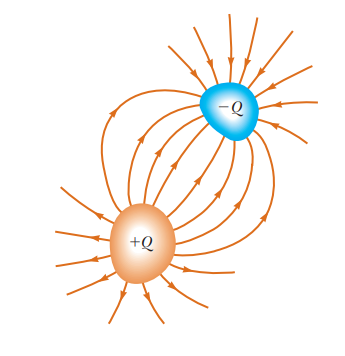
\includegraphics[width=0.4\linewidth]{images/figure1.png}
    \caption{Biểu diễn sơ đồ điện trường của một tụ điện bất kỳ, gồm hai vật dẫn mang điện lượng bằng nhau nhưng trái dấu ($+Q$ và $-Q$)}
    \label{fig:placeholder}
\end{figure}

\subsubsection{Định nghĩa}
Khi vật dẫn $B$ bao trùm hết vật dẫn $A$, ta tích cho vật dẫn $A$ một điện tích $+Q$, thì hai bề mặt trong và ngoài của vật dẫn $B$ sẽ tích điện $-Q$, $+Q$. Nối mặt ngoài cùng của vật dẫn $B$ xuống đất (mặt ngoài cùng trung hòa) ta có hai bề mặt kim loại tích điện trái dấu $-Q$, $+Q$ gọi là hai bản (cốt) của tụ điện.

\begin{figure}[H]
    \centering
    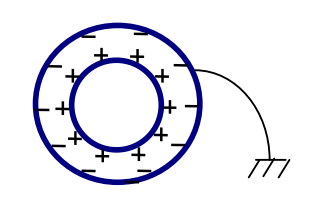
\includegraphics[width=0.5\linewidth]{images/figure2.png}
    \caption{Mô hình cấu tạo tụ điện: Vật dẫn bao ngoài được nối đất để triệt tiêu điện tích cùng dấu, tạo thành hai bản tụ mang điện tích trái dấu có độ lớn bằng nhau.}
    \label{fig:placeholder}
\end{figure}

\subsubsection{Điện dung của tụ điện}
Khi ta tích điện cho một tụ điện điện lượng $Q$, giữa hai bản tụ sẽ xuất hiện một hiệu điện thế $\Delta V$. Nếu tiếp tục tăng điện tích $Q$ thì hiệu điện thế $\Delta V$ cũng tăng theo tỉ lệ thuận tương ứng. Tuy nhiên, tỉ số giữa độ lớn điện tích $Q$ và hiệu điện thế $\Delta V$ luôn luôn là một hằng số đối với một tụ điện nhất định.

Hằng số này đặc trưng cho khả năng tích điện của tụ điện ở một hiệu điện thế cho trước, và được gọi là điện dung của tụ điện.

Biểu thức định nghĩa điện dung: 
$$C = \frac{Q}{\Delta V}$$

Trong đó: 
\begin{itemize}
\item $C$: Điện dung của tụ điện, có đơn vị là Farad (F).
\item $Q$: Độ lớn điện tích trên một bản tụ, có đơn vị là Coulomb (C).
\item $\Delta V$: Hiệu điện thế giữa hai bản tụ, có đơn vị là Volt (V).
\end{itemize}

\subsubsection{Tụ điện phẳng}
\begin{figure}[H]
    \centering
    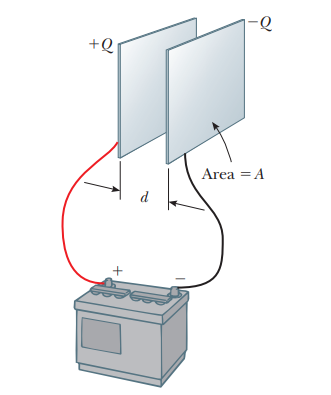
\includegraphics[width=0.4\linewidth]{images/figure3.png}
    \caption{Cấu tạo cơ bản của tụ điện phẳng: Hai bản kim loại có cùng diện tích bề mặt $A$, đặt cách nhau một khoảng $d$ và mang điện lượng trái dấu ($+Q$ và $-Q$) khi được nạp điện.}
    \label{fig:placeholder}
\end{figure}
Tụ điện phẳng là một trong những cấu trúc cơ bản và mang tính nền tảng nhất trong nghiên cứu tĩnh điện học. Cấu tạo không gian của hệ thống này bao gồm hai bản kim loại phẳng có cùng diện tích bề mặt $A$, được bố trí song song với nhau và ngăn cách bởi một khoảng cách $d$ trong môi trường chân không (hoặc không khí). Quá trình nạp điện cho hệ thống dẫn đến sự phân bố điện tích đối xứng, trong đó một bản mang điện tích dương $+Q$ và bản đối diện mang điện tích âm $-Q$. Hệ quả của quá trình này là sự hình thành mật độ điện tích mặt $\sigma$ trên bề mặt mỗi bản kim loại, được xác định bởi tỷ số giữa lượng điện tích và diện tích bề mặt tương ứng:
$$\sigma = \frac{Q}{A}$$

Trong các khảo sát lý thuyết, một giả thiết lý tưởng hóa thường được áp dụng là khoảng cách $d$ rất nhỏ so với kích thước tuyến tính của các bản tụ. Giả thiết này đóng vai trò quan trọng trong việc loại bỏ ảnh hưởng của hiệu ứng mép tại các rìa vật dẫn, cho phép xem xét điện trường $\vec{E}$ nội bộ giữa hai bản tụ là một điện trường đều, đồng thời coi điện trường ở không gian bên ngoài hệ thống xấp xỉ bằng $0$. Dựa trên cơ sở đó và thông qua việc áp dụng định lý Gauss, độ lớn của cường độ điện trường đều bên trong khoảng không gian giữa hai bản tụ được xác định chặt chẽ bằng biểu thức:
$$E = \frac{\sigma}{\epsilon_0} = \frac{Q}{\epsilon_0 A}$$
\textit{(Với $\epsilon_0$ là hằng số điện của chân không).}

Do đặc tính phân bố đều của điện trường nội bộ, độ giảm thế (hay hiệu điện thế $\Delta V$) giữa hai bản vật dẫn thể hiện mối quan hệ tuyến tính với chiều dài đường sức $d$. Mối liên hệ này được biểu diễn qua phương trình:
$$\Delta V = E \cdot d = \frac{Q \cdot d}{\epsilon_0 A}$$

Bằng cách tích hợp biểu thức hiệu điện thế này vào định nghĩa tổng quát của điện dung, biến số $Q$ được triệt tiêu, từ đó thiết lập được hệ thức toán học tính toán điện dung dành riêng cho cấu trúc tụ điện phẳng:
$$C = \frac{Q}{\Delta V} = \frac{\epsilon_0 A}{d}$$

Việc thiết lập phương trình giải tích trên đã minh chứng cho một nguyên lý vật lý cốt lõi: điện dung của một tụ điện phẳng mang tính chất nội tại và hoàn toàn độc lập với lượng điện tích $Q$ mà hệ đang lưu trữ hay hiệu điện thế $\Delta V$ được áp đặt lên nó. Thực chất, đại lượng này được quyết định hoàn toàn bởi các thông số cấu trúc không gian của hệ thống - tỷ lệ thuận với diện tích bề mặt bản tụ $A$, tỷ lệ nghịch với khoảng cách $d$ - và bản chất của môi trường điện môi tồn tại giữa hai bản cực.

\subsubsection{Sự phụ thuộc của điện dung vào các yếu tố hình học}
Từ biểu thức tính điện dung của tụ điện phẳng ($C = \frac{\epsilon_0 A}{d}$), ta có thể giải thích bản chất vật lý của sự phụ thuộc này thông qua các đặc điểm sau:
\begin{enumerate}
    \item Ảnh hưởng của diện tích bản tụ ($A$)\\
    Khi tụ điện được nạp điện từ một nguồn, các electron sẽ di chuyển và tích tụ trên bản cực âm, đồng thời bản cực dương mất đi một lượng electron tương ứng. Nếu diện tích bề mặt bản tụ $A$ càng lớn, không gian để điện tích phân bố càng rộng rãi. Điều này cho phép các bản tụ chứa được một lượng điện tích lớn hơn nhiều mà vẫn duy trì cùng một mức hiệu điện thế. Do đó, điện dung của tụ điện tỉ lệ thuận với diện tích bề mặt bản tụ ($C \propto A$).
    \item Ảnh hưởng của khoảng cách giữa hai bản tụ ($d$)\\
    Xét trường hợp tụ điện đang được duy trì kết nối với một nguồn điện (pin). Giả sử ta dịch chuyển để đưa hai bản tụ lại gần nhau (làm giảm khoảng cách $d$).
    \begin{itemize}
        \item Ngay tại khoảnh khắc dịch chuyển, lượng điện tích trên các bản tụ chưa kịp thay đổi tức thời, do đó cường độ điện trường $E$ giữa hai bản tạm thời giữ nguyên.
        \item Tuy nhiên, vì khoảng cách $d$ giảm, hiệu điện thế giữa hai bản tụ lúc này (tính theo công thức $\Delta V = E \cdot d$) sẽ bị suy giảm, trở nên nhỏ hơn hiệu điện thế của nguồn pin.
    \end{itemize}
\end{enumerate}

Sự chênh lệch điện áp này ngay lập tức tạo ra một điện trường dọc theo các dây nối, thúc đẩy dòng điện tích tiếp tục di chuyển từ nguồn vào tụ điện. Quá trình này làm tăng lượng điện tích $Q$ trên các bản tụ, kéo theo sự gia tăng hiệu điện thế giữa chúng. Dòng điện tích sẽ chỉ dừng lại khi hiệu điện thế của tụ điện phục hồi và cân bằng hoàn toàn với hiệu điện thế của pin.

Như vậy, thao tác đưa hai bản cực lại gần nhau đã giúp tụ điện gia tăng khả năng tích trữ điện tích ở cùng một mức điện áp. Ngược lại, nếu khoảng cách $d$ tăng lên, lượng điện tích lưu trữ sẽ giảm đi. Điều này giải thích bản chất vật lý của mối quan hệ tỉ lệ nghịch giữa điện dung $C$ và khoảng cách $d$ ($C \propto \frac{1}{d}$).

\subsection{Cường độ điện trường trong tụ điện phẳng}
\subsubsection{Định lý Gauss}
Định lý Gauss trong tĩnh điện học phát biểu rằng: Thông lượng điện trường gửi qua một mặt kín bất kỳ (gọi là mặt Gauss) bằng tổng đại số các điện tích nằm trọn bên trong mặt đó chia cho hằng số điện của chân không.

Biểu thức toán học:
$$\Phi_E = \oint \vec{E} \cdot d\vec{A} = \frac{q_{in}}{\epsilon_0}$$

Trong đó:
\begin{itemize}
    \item $\Phi_E$: Thông lượng điện trường qua mặt kín.
    \item $\vec{E}$: Vectơ cường độ điện trường tại vị trí vi phân diện tích.
    \item $q_{in}$: Tổng đại số các điện tích được bao bọc bên trong mặt Gauss.
    \item $\epsilon_0$: Hằng số điện của chân không.
\end{itemize}

Nguyên tắc chọn mặt Gauss:

Mặc dù định lý Gauss đúng với mọi mặt kín, nhưng trong thực hành, để tính toán cường độ điện trường $\vec{E}$ một cách dễ dàng, ta cần chọn một mặt Gauss phù hợp dựa trên tính đối xứng của sự phân bố điện tích. Bề mặt được chọn cần thỏa mãn ít nhất một trong các điều kiện sau đây để đơn giản hóa quá trình lấy tích phân:
\begin{enumerate}
    \item \textbf{Tính đối xứng về độ lớn:} Độ lớn cường độ điện trường $E$ không đổi tại mọi điểm trên bề mặt.
    \item \textbf{Điện trường vuông góc với mặt phẳng:} Vectơ điện trường $\vec{E}$ song song với vectơ diện tích $d\vec{A}$. Khi đó, biểu thức dưới dấu tích phân trở thành vô hướng: $\vec{E} \cdot d\vec{A} = E dA$.
    \item \textbf{Điện trường tiếp tuyến với mặt phẳng:} Vectơ điện trường $\vec{E}$ vuông góc với vectơ diện tích $d\vec{A}$. Khi đó, tích vô hướng triệt tiêu: $\vec{E} \cdot d\vec{A} = 0$.
    \item \textbf{Vùng không có điện trường:} Cường độ điện trường bằng không tại mọi điểm trên bề mặt xét ($E = 0$).
\end{enumerate}


\subsubsection{Xác định cường độ điện trường bằng định lý Gauss}
Để xác định cường độ điện trường trong tụ điện phẳng, quy trình tính toán được thực hiện qua hai giai đoạn: xác định điện trường do một bản phẳng đơn lẻ gây ra và áp dụng nguyên lý chồng chất cho hệ hai bản tụ.

\textbf{Cường độ điện trường của một bản phẳng tích điện}
    
Xét một bản kim loại phẳng vô hạn, tích điện đều với mật độ điện tích mặt $\sigma$. Chọn mặt Gauss là một hình trụ có trục vuông góc với bản tích điện và hai đáy song song với bản đó. Do tính đối xứng, vectơ cường độ điện trường $\vec{E}$ có hướng vuông góc với bản kim loại và độ lớn bằng nhau tại mọi điểm trên hai mặt đáy của hình trụ. Trong khi đó, thông lượng điện trường qua mặt xung quanh của hình trụ bằng không vì các đường sức song song với bề mặt này.

Áp dụng định lý Gauss, thông lượng điện trường chỉ đi qua hai mặt đáy, dẫn đến biểu thức xác định cường độ điện trường do một bản phẳng gây ra có độ lớn:
$$E = \frac{\sigma}{2\epsilon_0}$$

\textbf{Cường độ điện trường bên trong và bên ngoài tụ điện}

Xét mô hình tụ điện phẳng gồm hai bản kim loại song song mang điện tích trái dấu với mật độ $\sigma$ và $-\sigma$. Theo nguyên lý chồng chất, cường độ điện trường tại một điểm bất kỳ là tổng vectơ của điện trường do từng bản cực tạo ra.

\begin{itemize}
    \item \textbf{Vùng không gian giữa hai bản tụ:} Các vectơ điện trường do bản dương và bản âm gây ra có cùng phương và cùng hướng. Do đó, chúng cộng đại số với nhau, tạo ra điện trường bên trong tụ điện có độ lớn không đổi:
    $$E = \frac{\sigma}{2\epsilon_0} + \frac{\sigma}{2\epsilon_0} = \frac{\sigma}{\epsilon_0}$$
    \item \textbf{Vùng không gian bên ngoài tụ điện:} Vectơ điện trường do hai bản cực gây ra có cùng độ lớn nhưng ngược chiều nhau. Hệ quả là chúng triệt tiêu lẫn nhau, khiến cường độ điện trường ở vùng này xấp xỉ bằng không.
\end{itemize}

\textbf{Điều kiện áp dụng mô hình lý tưởng}

Các kết quả phân tích trên được thiết lập dựa trên mô hình tụ điện lý tưởng, trong đó thỏa mãn các điều kiện sau: diện tích của hai bản tụ đủ lớn để có thể coi là vô hạn, khoảng cách $d$ giữa hai bản rất nhỏ so với kích thước tuyến tính của chúng, và có thể bỏ qua hiệu ứng mép tại các rìa bản tụ.

\subsection{Năng lượng và mật độ năng lượng điện trường}
Việc tách biệt các điện tích dương và âm trong hệ thống hai vật dẫn của tụ điện đòi hỏi một công cơ học nhất định. Công này không mất đi mà được lưu trữ trong hệ thống dưới dạng năng lượng tiềm tàng, cụ thể là năng lượng tĩnh điện. Khi tụ điện được phóng điện thông qua một dây dẫn, năng lượng này sẽ được giải phóng, đôi khi có thể quan sát được dưới dạng tia lửa điện hoặc gây ra hiện tượng giật điện nếu tiếp xúc trực tiếp.

\begin{figure}
    \centering
    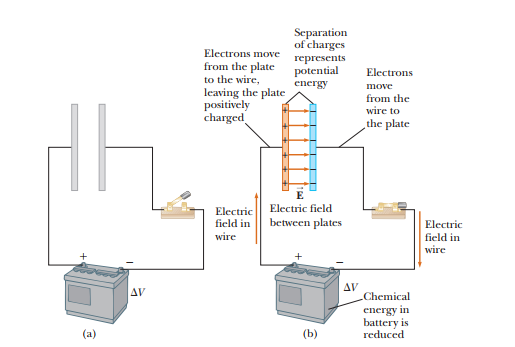
\includegraphics[width=0.7\linewidth]{images/figure4.png}
    \caption{Sơ đồ mô tả quá trình nạp điện và chuyển hóa năng lượng trong tụ điện phẳng: (a) Khi mạch hở; (b) Khi đóng công tắc, năng lượng hóa học từ pin chuyển hóa thành năng lượng điện thế thông qua sự phân tách các điện tích và thiết lập điện trường $\vec{E}$ giữa hai bản tụ.}
    \label{fig:placeholder}
\end{figure}
\subsubsection{Tính toán năng lượng lưu trữ trong tụ điện}
Để xác định tổng năng lượng tích lũy, ta xem xét quá trình nạp điện cho tụ điện như một chuỗi các bước dịch chuyển điện tích vi phân. Giả sử tại một thời điểm bất kỳ trong quá trình nạp, điện tích trên tụ điện là $q$ và hiệu điện thế tương ứng là $\Delta V$. Theo định nghĩa về điện dung, ta có mối liên hệ:
$$\Delta V = \frac{q}{C}$$

Khi một lượng điện tích vi phân $dq$ được chuyển từ bản mang điện thế thấp sang bản mang điện thế cao hơn, công vi phân $dW$ cần thực hiện để thắng lực điện trường là:
$$dW = \Delta V dq = \frac{q}{C}dq$$

Tổng công cần thiết để nạp điện cho tụ điện từ trạng thái không tích điện ($q=0$) đến khi đạt điện tích cuối cùng $Q$ được xác định bằng phép tính tích phân:
$$W = \int_{0}^{Q} \frac{q}{C} dq = \frac{1}{C} \int_{0}^{Q} q \, dq = \frac{Q^2}{2C}$$

\begin{figure}[H]
    \centering
    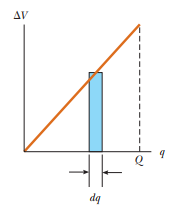
\includegraphics[width=0.35\linewidth]{images/figure5.png}
    \caption{Mối liên hệ tuyến tính giữa hiệu điện thế và điện tích của tụ điện. Tổng công thực hiện để nạp điện cho tụ đạt giá trị $Q$ tương ứng với diện tích hình tam giác nằm dưới đường thẳng $\Delta V(q)$.}
    \label{fig:placeholder}
\end{figure}

Vì công thực hiện bằng với năng lượng thế tĩnh điện $U$ tích lũy trong tụ điện, ta có các biểu thức tương đương để xác định năng lượng này:
$$U = \frac{Q^2}{2C} = \frac{1}{2}Q\Delta V = \frac{1}{2}C(\Delta V)^2$$

\subsubsection{Mật độ năng lượng điện trường}
Năng lượng trong tụ điện có thể được xem là lưu trữ trực tiếp trong điện trường tồn tại giữa hai bản cực. Đối với trường hợp tụ điện phẳng, ta có mối liên hệ giữa hiệu điện thế và cường độ điện trường là $\Delta V = Ed$, và điện dung $C = \frac{\epsilon_0 A}{d}$. Thay các giá trị này vào công thức năng lượng, ta thu được:
$$U = \frac{1}{2} \left( \frac{\epsilon_0 A}{d} \right) (Ed)^2 = \frac{1}{2} (\epsilon_0 Ad) E^2$$
Vì tích số $Ad$ chính là thể tích $V_{vol}$ của vùng không gian chứa điện trường, năng lượng trên mỗi đơn vị thể tích - gọi là mật độ năng lượng điện trường $u_E$ - được xác định như sau:
$$u_E = \frac{U}{Ad} = \frac{1}{2} \epsilon_0 E^2$$

Mặc dù biểu thức này được xây dựng dựa trên mô hình tụ điện phẳng, nó mang tính chất tổng quát và đúng cho bất kỳ điện trường nào trong chân không. Như vậy, mật độ năng lượng tại một điểm bất kỳ trong điện trường luôn tỷ lệ thuận với bình phương độ lớn cường độ điện trường tại điểm đó.

\subsection{Tụ điện phẳng có điện môi}
Chất điện môi là các vật liệu không dẫn điện, điển hình như cao su, thủy tinh hoặc giấy sáp. Việc đưa chất điện môi vào giữa các bản tụ không chỉ giúp ngăn cách vật lý giữa hai bản cực mà còn làm thay đổi đáng kể các đặc tính điện của hệ thống.
\subsubsection{Ảnh hưởng của điện môi lên điện dung}
\begin{figure}[H]
    \centering
    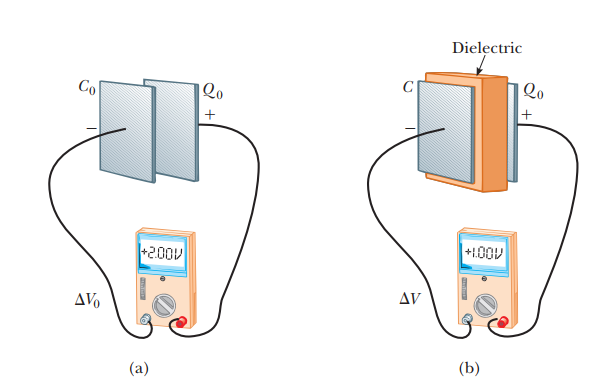
\includegraphics[width=0.6\linewidth]{images/figure6.png}
    \caption{Thí nghiệm minh họa ảnh hưởng của chất điện môi lên hiệu điện thế của tụ điện khi giữ nguyên điện lượng $Q_0$. (a) Hiệu điện thế ban đầu $\Delta V_0$ khi không có điện môi; (b) Hiệu điện thế $\Delta V$ giảm xuống sau khi chèn chất điện môi lấp đầy khoảng không gian giữa hai bản cực.}
    \label{fig:placeholder}
\end{figure}
Để khảo sát tác dụng của chất điện môi, xét một tụ điện phẳng đã được nạp điện lượng $Q_0$ và sau đó ngắt khỏi nguồn. Tại trạng thái ban đầu trong chân không, tụ điện có điện dung $C_0$ và hiệu điện thế đo được giữa hai bản tụ là $\Delta V_0 = Q_0/C_0$.

Khi chèn một tấm điện môi lấp đầy khoảng không gian giữa hai bản cực, thực nghiệm cho thấy hiệu điện thế giữa chúng giảm xuống một giá trị $\Delta V$ mới. Mối liên hệ giữa hiệu điện thế trước và sau khi có điện môi được xác định qua hệ số không thứ nguyên $\kappa$:
$$\Delta V = \frac{\Delta V_0}{\kappa}$$

Vì hệ thống đã được ngắt khỏi nguồn nên điện tích $Q_0$ trên các bản cực không thay đổi. Do đó, giá trị điện dung của tụ điện khi có điện môi phải thay đổi tương ứng:
$$C = \frac{Q_0}{\Delta V} = \frac{Q_0}{\Delta V_0 / \kappa} = \kappa \frac{Q_0}{\Delta V_0}$$
Hay:
$$C = \kappa C_0$$

Trong đó, $\kappa$ được gọi là hằng số điện môi của vật liệu. Vì thực nghiệm cho thấy $\Delta V < \Delta V_0$, ta luôn có $\kappa > 1$, nghĩa là việc chèn chất điện môi luôn làm tăng điện dung của tụ điện. Đối với mô hình tụ điện phẳng, biểu thức tính điện dung tổng quát khi có điện môi được xác định bởi:
$$C = \kappa \frac{\epsilon_0 A}{d}$$

\subsubsection{Giới hạn vật lý và điện áp định mức}
Mặc dù việc giảm khoảng cách $d$ hoặc tăng hằng số điện môi $\kappa$ có thể làm tăng điện dung, nhưng trong thực tế, các tham số này bị giới hạn bởi hiện tượng đánh thủng điện môi. Với mỗi loại vật liệu, tồn tại một giá trị cường độ điện trường tối đa mà nó có thể chịu đựng được trước khi mất tính cách điện và trở nên dẫn điện, gọi là độ bền điện môi.

Hệ quả là các tụ điện thực tế luôn đi kèm với thông số điện áp định mức (hoặc điện áp đánh thủng). Thông số này đại diện cho mức hiệu điện thế lớn nhất có thể đặt vào tụ điện mà không gây ra sự phóng điện xuyên qua lớp điện môi. Do đó, khi thiết kế và lựa chọn tụ điện cho các ứng dụng cụ thể, người kỹ sư cần phải xem xét đồng thời cả giá trị điện dung và giới hạn điện áp hoạt động để đảm bảo an toàn và độ bền cho hệ thống.

% \input{section/methodology_implementation}
% \input{section/experience_result}
% \input{section/discussion}
% \section{Kết luận và mở rộng}

\subsection{Kết quả đạt được}
Bài tập lớn đã hoàn thành đầy đủ các mục tiêu đề ra:
\begin{enumerate}
    \item Thiết lập và giải thành công hệ phương trình vi phân bậc 2 mô tả chuyển động ném xiên có lực cản tuyến tính, sử dụng thư viện SymPy cho lời giải symbolic chính xác.
    
    \item Tính toán và phân tích chi tiết 5 khía cạnh:
    \begin{itemize}
        \item Quỹ đạo $y(x)$ cho 5 góc ném khác nhau ($15°$, $30°$, $45°$, $60°$, $75°$)
        \item So sánh định lượng quỹ đạo có và không có lực cản
        \item Biến thiên vận tốc $v_x(t)$, $v_y(t)$ theo thời gian
        \item Biến thiên năng lượng (động năng, thế năng, cơ năng, năng lượng mất)
        \item Ảnh hưởng của hệ số cản $h$ đến quỹ đạo
    \end{itemize}
    
    \item Xây dựng ứng dụng web tương tác (Streamlit + Plotly) cho phép nhập tham số bằng slider và quan sát kết quả biến đổi theo thời gian thực.
\end{enumerate}

\subsection{Nhận xét vật lý quan trọng}
Từ kết quả mô phỏng, có thể rút ra các kết luận vật lý quan trọng sau:

\begin{enumerate}
    \item Lực cản tuyến tính $\vec{F}_c = -h\vec{v}$ làm quỹ đạo \textbf{mất tính đối xứng parabol}: nhánh đi xuống dốc hơn nhánh đi lên do vận tốc ngang suy giảm theo hàm mũ.
    
    \item \textbf{Góc ném tối ưu} (cho tầm xa cực đại) dịch chuyển về phía nhỏ hơn $45°$. Trong điều kiện mô phỏng ($h = 0.5$ kg/s), góc tối ưu $\approx 30°$.
    
    \item Vận tốc ngang giảm theo $e^{-ht/m}$, vận tốc đứng tiến tới \textbf{vận tốc giới hạn} $v_\infty = -mg/h$, phù hợp với lý thuyết vật lý.
    
    \item \textbf{Cơ năng không bảo toàn} do lực cản là lực không bảo toàn, luôn sinh công âm. Năng lượng cơ học chuyển hóa thành nhiệt năng.
    
    \item Hệ số cản $h$ ảnh hưởng \textbf{phi tuyến} đến quỹ đạo -- tầm xa giảm rất nhanh khi $h$ tăng.
\end{enumerate}

\subsection{So sánh lý thuyết và mô phỏng}
Nghiệm giải tích từ SymPy khớp hoàn toàn với lý thuyết vật lý:
\begin{itemize}
    \item Khi $h \to 0$: nghiệm hội tụ về dạng parabol cổ điển (phương trình \ref{eq:ideal}).
    \item Khi $t \to \infty$: $v_x \to 0$, $v_y \to -mg/h$ (vận tốc giới hạn).
    \item Năng lượng: $E_0 = KE + PE + W_{cản}$ luôn thỏa mãn tại mọi thời điểm, xác nhận tính nhất quán của mô hình.
\end{itemize}

\subsection{Hướng mở rộng}
Một số hướng phát triển tiềm năng nếu muốn nâng cao độ chính xác của mô hình:
\begin{itemize}
    \item \textbf{Lực cản bậc hai:} $\vec{F}_{cản} = -c|\vec{v}|\vec{v}$, phù hợp hơn với vận tốc cao. Mô hình này không có nghiệm giải tích đơn giản, cần sử dụng phương pháp Runge-Kutta (\texttt{scipy.integrate.solve\_ivp}).
    \item \textbf{Hiệu ứng gió:} Thêm thành phần lực ngoài theo phương ngang.
    \item \textbf{Mô phỏng 3D:} Mở rộng sang không gian 3 chiều.
    \item \textbf{Tối ưu hóa góc ném:} Sử dụng \texttt{scipy.optimize} để tìm góc cho tầm xa cực đại ứng với mỗi bộ tham số.
\end{itemize}

\newpage

\nocite{serway2008physics}
\bibliographystyle{ieeetr}
\bibliography{references}

\newpage
\appendix
\begin{landscape}
\section{Phụ lục}
% Bắt đầu môi trường xoay ngang trang giấy

\thispagestyle{empty} % Lệnh xóa Header và Footer cho trang này

\subsection{Bảng phân công nhiệm vụ và tiến độ nhóm}
\begin{center}
\renewcommand{\arraystretch}{1.5}
% Đã xóa 1 cột 'c' trong khai báo định dạng và nới phần còn lại
\begin{tabularx}{\linewidth}{|c|p{2.5cm}|c|X|*{5}{>{\centering\arraybackslash}p{1.2cm}|}}
\hline
\textbf{STT} & \textbf{Họ tên} & \textbf{MSSV} & \textbf{Công việc thực hiện} & \textbf{T1} & \textbf{T2} & \textbf{T3} & \textbf{T4} & \textbf{T5} \\ \hline
1 & Trần Nguyễn Phương Tuyền  & 213833 & Viết Ch.1; Điều phối nhóm, review báo cáo. & Viết Ch.1 & Hoàn thiện & Review mô phỏng & Sửa báo cáo & Tập thuyết trình \\ \hline
2 & Võ Thanh Quân & 2114562 & Viết Ch.1; Viết Ch.4 (So sánh \& mở rộng). & Viết Ch.1 & Hoàn thiện & So sánh LT-MP & Viết ứng dụng & Tập thuyết trình \\ \hline
3 & Trần Đăng Bảo & 2210270 & Code Python mô phỏng tụ lý tưởng \& điện môi. & Nghiên cứu & Code tụ lý tưởng & Code tụ điện môi & Hoàn thiện đồ thị & Tập thuyết trình \\ \hline
4 & Thịnh Trần Khánh Linh  & 2211862 & Code Python mô phỏng tụ lý tưởng \& điện môi. & Nghiên cứu & Code tụ lý tưởng & Code tụ điện môi & Khảo sát tham số & Tập thuyết trình \\ \hline
5 & Mai Trần Thiên Ân  & 2310181 & Viết Chương 3 – Phân tích kết quả mô phỏng. & Đọc tài liệu & Phân tích tụ lý tưởng & Phân tích điện môi & Hoàn thiện & Tập thuyết trình \\ \hline
6 & Nguyễn Quốc Trạng  & 2213565 & Viết Chương 3 – Phân tích kết quả mô phỏng. & Đọc tài liệu & Phân tích tụ lý tưởng & Phân tích điện môi & Hoàn thiện & Tập thuyết trình \\ \hline
7 & Trần Minh Khôi  & 2311703 & Viết Ch.4; Tổng hợp báo cáo; Làm Slide. & Tạo template & Chèn Ch.1 & Chèn Ch.2 & Tổng hợp \& Slide & Tập thuyết trình \\ \hline
\end{tabularx}
\captionof{table}{Bảng phân công thực hiện bài tập lớn}
\end{center}

\vspace{0.8cm}

\subsection{Phân nhóm nội dung chi tiết}
\thispagestyle{empty}
\begin{center}
\renewcommand{\arraystretch}{1.5}
\begin{tabular}{|l|l|p{14cm}|} 
\hline
\textbf{Nội dung} & \textbf{Phụ trách} & \textbf{Chi tiết công việc} \\ \hline
Chương 1 & Trần Nguyễn Phương Tuyền + Võ Thanh Quân & Dẫn giải công thức định lý Gauss, năng lượng, mật độ năng lượng, ảnh hưởng điện môi. \\ \hline
Chương 2 & Trần Đăng Bảo + Thịnh Trần Khánh Linh & Code Python: đồ thị 3D $w(x,y)$, 2D $w(z)$, so sánh có/không điện môi, khảo sát $W(d, V, \epsilon)$. \\ \hline
Chương 3 & Mai Trần Thiên Ân + Nguyễn Quốc Trạng & Giải thích vật lý: phân bố năng lượng đều, sự suy giảm khi có điện môi, ảnh hưởng tham số. \\ \hline
Chương 4 & Võ Thanh Quân + Trần Minh Khôi & So sánh sai số lý thuyết - mô phỏng, nhận xét ứng dụng thực tiễn của tụ điện. \\ \hline
Tổng hợp & Trần Đăng Bảo & Format bố cục, chú thích hình/bảng, TLTK IEEE, slide thuyết trình. \\ \hline
\end{tabular}
\end{center}

\end{landscape}
% Kết thúc môi trường xoay ngang

% \begin{thebibliography}{99}



% \end{thebibliography}


\end{document}

